%% file: template.tex = LaTeX template for article-like report 
%% init: sometime 1993
%% last: Feb  8 2015  Rob Rutten  Deil
%% site: http://www.staff.science.uu.nl/~rutte101/rrweb/rjr-edu/manuals/student-report/

%% First read ``latex-bibtex-simple-manual.txt'' at
%% http://www.staff.science.uu.nl/~rutte101/Report_recipe.html

%% Start your report production by copying this file into your XXXX.tex.
%% Small changes to the header part will make it an A&A or ApJ manuscript.

%%%%%%%%%%%%%%%%%%%%%%%%%%%%%%%%%%%%%%%%%%%%%%%%%%%%%%%%%%%%%%%%%%%%%%%%%%%%
\documentclass{aa}   %% Astronomy & Astrophysics style class
\usepackage{graphicx,natbib,url,twoopt}
\usepackage[varg]{txfonts}           %% A&A font choice
\usepackage{hyperref}                %% for pdflatex
%%\usepackage[breaklinks]{hyperref}  %% for latex+dvips
%%\usepackage{breakurl}              %% for latex+dvips
\usepackage{pdfcomment}              %% for popup acronym meanings
\usepackage{acronym}                 %% for popup acronym meanings

\hypersetup{
  colorlinks=true,   %% links colored instead of frames
  urlcolor=blue,     %% external hyperlinks
  linkcolor=red,     %% internal latex links (eg Fig)
}

\bibpunct{(}{)}{;}{a}{}{,}    %% natbib cite format used by A&A and ApJ

\pagestyle{plain}   %% undo the fancy A&A pagestyle 

%% Add commands to add a note or link to a reference
\makeatletter
\newcommand{\bibnote}[2]{\@namedef{#1note}{#2}}
\newcommand{\biblink}[2]{\@namedef{#1link}{#2}}
\makeatother

%% Commands to make citations ADS clickers and to add such also to refs
%% May 2014: they give error stops ("Illegal parameter number ..."}
%%   for plain latex with TeX Live 2013; the ad-hoc fixes added below let
%%   latex continue instead of stop within these commands.
%%   Please let me know if you know a better fix!
%%   No such problem when using pdflatex.
\makeatletter
 \newcommandtwoopt{\citeads}[3][][]{%
   \nonstopmode%              %% fix to not stop at error message in latex
   \href{http://adsabs.harvard.edu/abs/#3}%
        {\def\hyper@linkstart##1##2{}%
         \let\hyper@linkend\@empty\citealp[#1][#2]{#3}}%   %% Rutten, 2000
   \biblink{#3}{\href{http://adsabs.harvard.edu/abs/#3}{ADS}}%
   \errorstopmode}            %% fix to resume stopping at error messages 
 \newcommandtwoopt{\citepads}[3][][]{%
   \nonstopmode%              %% fix to not stop at error message in latex
   \href{http://adsabs.harvard.edu/abs/#3}%
        {\def\hyper@linkstart##1##2{}%
         \let\hyper@linkend\@empty\citep[#1][#2]{#3}}%     %% (Rutten 2000)
   \biblink{#3}{\href{http://adsabs.harvard.edu/abs/#3}{ADS}}%
   \errorstopmode}            %% fix to resume stopping at error messages
 \newcommandtwoopt{\citetads}[3][][]{%
   \nonstopmode%              %% fix to not stop at error message in latex
   \href{http://adsabs.harvard.edu/abs/#3}%
        {\def\hyper@linkstart##1##2{}%
         \let\hyper@linkend\@empty\citet[#1][#2]{#3}}%     %% Rutten (2000)
   \biblink{#3}{\href{http://adsabs.harvard.edu/abs/#3}{ADS}}%
   \errorstopmode}            %% fix to resume stopping at error messages 
 \newcommandtwoopt{\citeyearads}[3][][]{%
   \nonstopmode%              %% fix to not stop at error message in latex
   \href{http://adsabs.harvard.edu/abs/#3}%
        {\def\hyper@linkstart##1##2{}%
         \let\hyper@linkend\@empty\citeyear[#1][#2]{#3}}%  %% 2000
   \biblink{#3}{\href{http://adsabs.harvard.edu/abs/#3}{ADS}}%
   \errorstopmode}            %% fix to resume stopping at error messages 
\makeatother

%% Acronyms
\newacro{ADS}{Astrophysics Data System}
\newacro{NLTE}{non-local thermodynamic equilibrium}
\newacro{NASA}{National Aeronautics and Space Administration}

%% Add popups with meaning to acronyms 
%% NB: only show up in Adobe Reader and do not work with \input or \include
\gdef\acp#1{%
  \pdfmarkupcomment[markup=Underline,color={1 1 1},author={{#1}},opacity=0]%
  {{#1}}{{\acl{#1}}}}

%% Spectral species
\def\MgI{\ion{Mg}{I}}          %% A&A; for aastex use \def\MgI{\ion{Mg}{1}} 
\def\MgII{\ion{Mg}{II}}        %% A&A; for aastex use \def\MgII{\ion{Mg}{2}} 

%% Hyphenation
\hyphenation{Schrij-ver}       %% Dutch ij is a single character

%%%%%%%%%%%%%%%%%%%%%%%%%%%%%%%%%%%%%%%%%%%%%%%%%%%%%%%%%%%%%%%%%%%%%%%%%%%%
\begin{document}  

%% simple header.  Change into A&A or ApJ commands for those journals

\twocolumn[{%
\vspace*{4ex}
\begin{center}
  {\Large \bf Project 2, Schrödinger's equation for two electrons in a three-dimensional harmonic oscillator well}\\[4ex]
  {\large \bf Andreas Ellewsen, Peder Forfang}\\[4ex]
  %{\large \bf Andreas Ellewsen$^{1}$}\\[4ex]
  %\begin{minipage}[t]{15cm}
  %      $^1$ Institute of theoretical astrophysics\\

%  {\bf Abstract.} We learned how to write nice reports \ldots 

  %\vspace*{2ex}
  %\end{minipage}
\end{center}
}] 

%%%%%%%%%%%%%%%%%%%%%%%%%%%%%%%%%%%%%%%%%%%%%%%%%%%%%%%%%%%%%%%%%%%%%%%%%%%%
\section{Introduction}   \label{sec:Intro}
%%%%%%%%%%%%%%%%%%%%%%%%%%%%%%%%%%%%%%%%%%%%%%%%%%%%%%%%%%%%%%%%%%%%%%%%%%%%
The aim of this project is to solve Schrödinger's equation for two electrons in a harmonic oscillator potential, with, and without a repulsive Couloumb interaction. This is done using the Jacobi rotation method. First for one electron in a harmonic oscillator potential to test the precission of the method, and then for both variations with two electrons.
%%%%%%%%%%%%%%%%%%%%%%%%%%%%%%%%%%%%%%%%%%%%%%%%%%%%%%%%%%%%%%%%%%%%%%%%%%%%
\section{Discretizing the wave equation}    \label{sec:Discretizing}
%%%%%%%%%%%%%%%%%%%%%%%%%%%%%%%%%%%%%%%%%%%%%%%%%%%%%%%%%%%%%%%%%%%%%%%%%%%%
To solve this using the Jacobi method, we first have to discretize the equation and rewrite it to a square matrix.
The radial part of the wave equation for a single electron in a harmonic oscillator potential reads
\begin{equation}\label{Waveequation}
 -\frac{\hbar^2}{2m}\bigg(\frac{1}{r^2}\frac{d}{dr}r^2\frac{d}{dr} - \frac{l(l+1)}{r^2}\bigg)R(r) + V(r)R(r) = ER(r).
\end{equation}
In our case $V = 1/2 kr^2$, with $k = m\omega^2$, and 
\begin{equation}
\label{Energy}
E_{nl} = \hbar\omega \bigg(2n + l +\frac{3}{2}\bigg).
\end{equation}
Here $E_{nl}$ is the energy of the harmonic oscillator in three dimensions, and $n = 0,1,2,...$, $l = 0,1,2,...$. In this project we will use $l = 0$. We introduce the dimensional less variable $\rho = r/\alpha$ where $\alpha$ is a constant with dimension length. Rewriting equation \ref{Waveequation} we end up with

\begin{equation}\label{dimensionless}
  -\frac{d^2}{d\rho^2} u(\rho) + \rho^2u(\rho)  = \lambda u(\rho). 
\end{equation}

where 
\begin{equation}
\lambda = \frac{2m\alpha^2}{\hbar^2}E,
\end{equation}

and 

\begin{equation}
\alpha = \left(\frac{\hbar^2}{mk}\right)^{1/4}.
\end{equation}
If we now use that the second derivative of a function $u$ can be written
\begin{equation}
    u''=\frac{u(\rho+h) -2u(\rho) +u(\rho-h)}{h^2} +O(h^2),
\end{equation}
where $h$ is our step length, defined as 
\begin{equation}
 h = \frac{\rho_{max}-\rho_{min}}{n_{step}}
\end{equation}
giving us 
\begin{equation}
 \rho_i = \rho_{min} +ih~,~i=0,1,2,...,n_{step}.
\end{equation}
Using this we can rewrite equation \ref{dimensionless} to the discretized form
\begin{equation}
 -\frac{u_{i+1} -2u_i +u_{i-1} }{h^2}+V_iu_i  = \lambda u_i
\end{equation}
which is the one we will be using. Solving this numerically, we will define a tridiagonal matrix where 

\begin{equation}
 d_i=\frac{2}{h^2}+V_i
\end{equation}

is the diagonal elements, and

\begin{equation}
 e_i=-\frac{1}{h^2}
\end{equation}

is the non-diagonal elements. Finally we can rewrite the Schrödinger equation to

\begin{equation}
 d_iu_i+e_{i-1}u_{i-1}+e_{i+1}u_{i+1}  = \lambda u_i.
\end{equation}

This is the equation we will be using Jacobi's method on.
%%%%%%%%%%%%%%%%%%%%%%%%%%%%%%%%%%%%%%%%%%%%%%%%%%%%%%%%%%%%%%%%%%%%%%%%%%%%
\section{Solving the discretized wave equation with Jacobi's method}   \label{sec:Saha}
%%%%%%%%%%%%%%%%%%%%%%%%%%%%%%%%%%%%%%%%%%%%%%%%%%%%%%%%%%%%%%%%%%%%%%%%%%%%
To solve this we make a program in c++ implementing Jacobi's method.
The program can be seen in the github repository linked in the references.

We compare our result with the analytical solutions of the eigenvalues. The lowest solutions are 3, 7 and 11. To get a 4 digit precission of the lowest three, we need $n_{step} = 200$. The eigenvalues depend on the value of $\rho_{max}$, which is expected as $\rho_{max}$ is the maximum distance from the potential well. In our computation we find that the solutions with $\rho_{max} = 5$ fits well with the analytical solutions. The number of similarity transformations needed before the non-diagonal elements in the matrix are essensially zero depend on how many $n_{step}$ we choose. With the 4 digit precission we reach a number of 71168 iterations. Trial and error for different values of $n$ reveals that the number of iterations is proportional to $n^2$. More precisely the number of iterations needed is approximately $7n^2/4$.

Comparing our algorithm to the one in the armadillo library reveals that the two methods produce exactly the same results. However the armadillo solver is a lot faster than our method. For $n = 100$, our method uses $1.20562$ seconds, while armadillo uses $0.004314$ seconds.

Next we will study two electrons in a harmonic oscillator well which also interact via a repulsive Couloumb interaction. Setting up the equation for this results in
\begin{equation}\label{Two electrons}
 \left(  -\frac{\hbar^2}{2 m} \frac{d^2}{dr_1^2} -\frac{\hbar^2}{2 m} \frac{d^2}{dr_2^2}+ \frac{1}{2}k r_1^2+ \frac{1}{2}k r_2^2\right)u(r_1,r_2)  = E^{(2)} u(r_1,r_2).
\end{equation}
To make this mess look nicer we change coordinates to the center of mass coordinate $R$, and make the equation dimensionless by multiplying with some constants, arriving at the final equation for the system
\begin{equation}\label{new potential}
   -\frac{d^2}{d\rho^2} \psi(\rho) + \omega_r^2\rho^2\psi(\rho) +\frac{1}{\rho} = \lambda \psi(\rho),
\end{equation}
where 
\begin{equation*}
 \omega_r^2=\frac{1}{4}\frac{mk}{\hbar^2} \alpha^4~,~\alpha = \frac{\hbar^2}{m\beta e^2}~,~\lambda = \frac{m\alpha^2}{\hbar^2}E.
\end{equation*}
Looking at equation \ref{new potential} we see that we will be solving the same equation again, only this time the potential term takes on a different form. This means that we can reuse our code from the one electron case to this one.

We treat $\omega_r$ as a strength parameter for the oscillator potential, and will study our case for different values of $\omega_r$. The lowest energies for the different $\omega$ values are tabulated in table \ref{Eigenvalues}. Studying the table shows that the excitation energies increase with higher $\omega$, which is logical since the potential is proportional with $\omega$. The potenital well gets deeper with higher oscillator strength, making it harder to get out of the potential.
The results in table \ref{Eigenvalues} are for $n = 1000$. Note that $\rho_{max}$ is varied depending on the value of $\omega_r$ since larger $\omega_r$ makes the potential narrower, making it unnecessary to calculate values for large $\rho$. 
\begin{table}
%\begin{center}
\begin{tabular}{| c | c | c | c | c |}
\hline
State & $\omega_r = 0.01$ & $\omega_r = 0.5$ & $\omega_r = 1$ & $\omega_r = 5$\\
\hline
1 & $0.105775$ & $2.23009$& $4.05784$ & $17.4484$\\
\hline
2 & $0.141508$ & $4.13433$& $7.90952$ & $37.0704$\\
\hline
3 & $0.177961$ & $6.0736$& $11.8188$ & $56.8505$\\
\hline
$\rho_{max}$ & 60 & 20 &10 &6 \\
\hline
\end{tabular}
%\end{center}
\caption{Excitation energy of the three lowest states in eV.}
\label{Eigenvalues}
\end{table}

In this case there exists good approximations to the analytical solutions. It can be shown that an apporixmation can be written
\begin{equation}
 \epsilon_m = 3\bigg(\frac{\omega_r}{2}\bigg)^{2/3} + \sqrt{3} \omega_r
\end{equation}

\begin{table}
%\begin{center}
\begin{tabular}{| c | c | c | c | c |}
\hline
State & $\omega_r = 0.01$ & $\omega_r = 0.5$ & $\omega_r = 1$ & $\omega_r = 5$\\
\hline
1 & $0.105041$ & $2.05658$& $3.62193$ & $14.1863$\\
\hline
2 & $0.139682$ & $3.78863$& $7.08603$ & $31.5068$\\
\hline
3 & $0.174323$ & $5.52068$& $10.5501$ & $48.8273$\\
\hline
\end{tabular}
%\end{center}
\caption{Analytical approximation of excitation energy of the three lowest states in eV.}
\label{Analytical}
\end{table}

Table \ref{Analytical} shows the analytical apporixmation of the eigenvalues. Comparing this to our numerical solutions we can see that they are quite coherent. This bodes well for our selfesteem and our numerical code.

%\begin{center}
\begin{figure}
 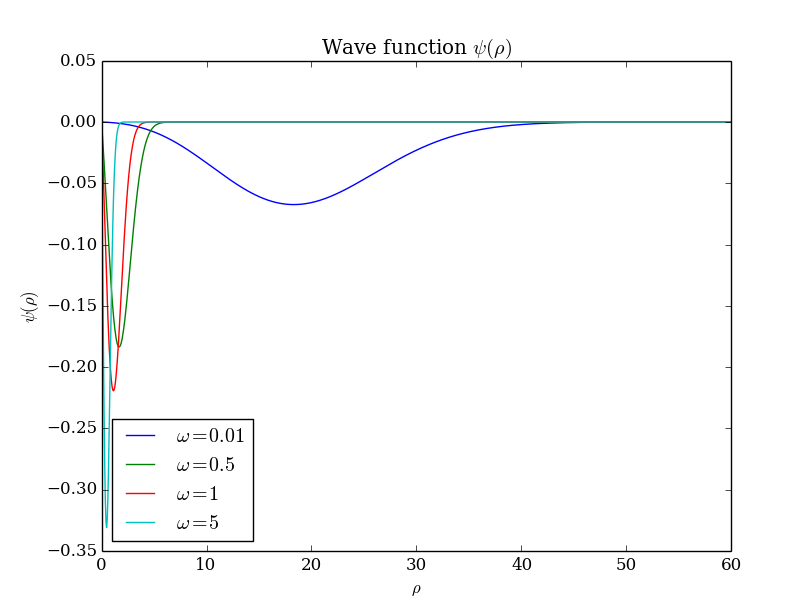
\includegraphics[width=.49\textwidth]{wave_func2.png}
\caption{Wavefunction with different $\omega_r$.}
 \label{wave_func}
 \end{figure}
%\end{center}

%\begin{center}
\begin{figure}
 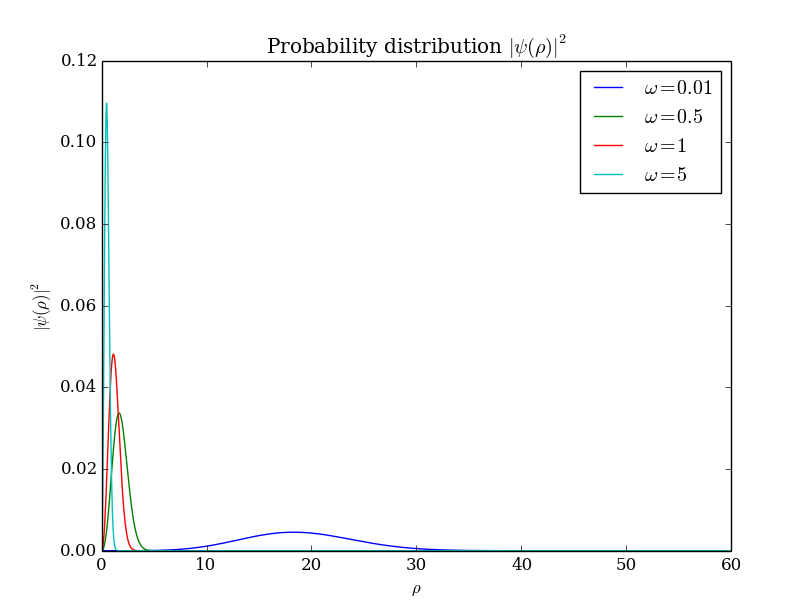
\includegraphics[width=.49\textwidth]{probability_func2.png}
\caption{Probability distribution of $\psi$.}
 \label{probability_func}
 \end{figure}
%\end{center}

Figure \ref{wave_func} shows the wavefunction for different $\omega_r$, while figure \ref{probability_func} shows the probability distribution. Here $\rho$ represents the coordinate of the mass center of the two electrons. As $\omega_r$ increases, the probability of finding the mass center in the potenital well increases. In short, bigger $\omega$ gives a deeper well, which in turn increases the probability that the electrons are located in the potential well. Meaning that by increasing $\omega_r$ we can constrain the distance between the two electrons to some probable range.

%%%%%%%%%%%%%%%%%%%%%%%%%%%%%%%%%%%%%%%%%%%%%%%%%%%%%%%%%%%%%%%%%%%%%%%%%%%%
\section{Testing} \label{sec:testing}
%%%%%%%%%%%%%%%%%%%%%%%%%%%%%%%%%%%%%%%%%%%%%%%%%%%%%%%%%%%%%%%%%%%%%%%%%%%%
As a final insurance that our code works the desired way, we will utilize some tests to make sure our code is coherent with mathematical laws and regulations. We know that if we set $n = 2$ then the program should complete in 1 itteration. We also know that the eigenvectors we find should all be orthogonal. Mathematically this means that we can take the dot product of them all and this should be equal to zero. 

Running the code with $n = 2$ does in fact complete the calculation in 1 iteration as it should.
To calculate whether the eigenvectors are orthogonal we set a tollerance of $10^-4$ and say that if the dot product of two vectors is smaller than this tollerance the dot product is zero. The reason we need to do this is because  we never get precisely zero when adding things together on a computer. When looking at the 3 first eigenvectors with $n = 1000$,$rho_{max} = 50$, and the potential corresponding to two electrons with repulsion, the code passes this test.

%%%%%%%%%%%%%%%%%%%%%%%%%%%%%%%%%%%%%%%%%%%%%%%%%%%%%%%%%%%%%%%%%%%%%%%%%%%%
\section{Conclusions} \label{sec:conclusions}
%%%%%%%%%%%%%%%%%%%%%%%%%%%%%%%%%%%%%%%%%%%%%%%%%%%%%%%%%%%%%%%%%%%%%%%%%%%%
In this project we have seen that we can use the Jacobi method to calculate the wavefunction of one electron in a potential well and two electrons in another potential well with repulsion. 
For the first case we saw that armadillo is much more effective than our method, and provides the same solution. Our approach came quite close to the analytical solutions, but it demanded a lot of steps leading to many iterations and thus long computation time. Nevertheless the numerical approximation was very close to the analytical solution.
We also saw that the method works well for two electrons in a potential well with Couloumb repulsion between them.
In this case $\rho_{max}$ has been set to different values for different $\omega_r$. This needed to be done because the solutions were highly dependent on both stepsize and $\rho_{max}$. Looking at the graphs for the wavefunctions revealse clearly why there is no point using very high $\rho_{max}$ for high $\omega_r$.

In conclusion we have seen that the jacobi rotation method works well for finding eigenvalues, and -vectors for quantum mechanical problems.

%%%%%%%%%%%%%%%%%%%%%%%%%%%%%%%%%%%%%%%%%%%%%%%%%%%%%%%%%%%%%%%%%%%%%%%%%%%%
\section{Source code}\label{sec:source}
%%%%%%%%%%%%%%%%%%%%%%%%%%%%%%%%%%%%%%%%%%%%%%%%%%%%%%%%%%%%%%%%%%%%%%%%%%%%
The source code for this document, the c++ project, and the python file for plotting can be found at \url{https://github.com/tellewsen/Project2}.



%%%%%%%%%%%%%%%%%%%%%%%%%%%%%%%%%%%%%%%%%%%%%%%%%%%%%%%%%%%%%%%%%%%%%%%%%%%%
%\begin{acknowledgements}
%\end{acknowledgements}

%%%%%%%%%%%%%%%%%%%%%%%%%%%%%%%%%%%%%%%%%%%%%%%%%%%%%%%%%%%%%%%%%%%%%%%%%%%%
%% references
\section{References}
M. Taut, Phys. Rev. A 48, 3561 - 3566 (1993)

%\bibliographystyle{aa-note} %% aa.bst but adding links and notes to references
%\raggedright              %% only for adsaa with dvips, not for pdflatex
%\bibliography{XXX}          %% XXX.bib = your Bibtex entries copied from ADS

\end{document}